\subsubsection{Fernsteuerung}
\label{subsubsec:fernsteuerung}
%todo fernbedienung in fernsteuerung

Der \gls{go1} lässt sich auf vier verschiedene Arten fernsteuern:

\begin{itemize}
    \item Fernbedienung
    \item App
    \item Webinterface
    \item Folgefunktion
\end{itemize}

\noindent Dieses Kapitel beschreibt alle vier Möglichkeiten kurz und zeigt diverse Limitierungen der einzelnen Umsetzungen auf.
Für alle vier Steuermöglichkeiten muss der Roboter angeschaltet und der Sportmodus aktiviert sein.
Sollte der Sportmodus nicht aktiviert sein und eine Verbindung auf den Raspberry Pi nicht möglich oder erwünscht sein,
so kann dieser über die gekoppelte Fernbedienung und der Tastenkombination \texttt{L2+START} aktiviert werden.
Der \gls{go1} muss sich hierfür in der Ausgangsposition wie in Kapitel \ref{subsubsec:inbetriebnahme_akku} beschrieben befinden.

\myparagraph{Fernbedienung}

Der Lieferumfang des \gls{go1} umfasst zwei physische Fernbedienungen, mit denen der Roboter gesteuert werden kann.
Die Hauptfernbedienung besitzt zwei sogenannte Joysticks, welche die Position und Bewegung Roboter in verschiedenen Achsen
manipulieren können.
Die zweite Fernbedienung, von Unitree \emph{Label Controller} genannt, besitzt lediglich ein Joystick, welches die Bewegung
nach vorne, hinten, links und rechts steuern kann.
Sie dient ebenfalls als Sender für die \emph{Folge}-Funktion.
Abbildung \ref{fig:controller} zeigt links die Hauptfernbedienung und rechts den Label-Controller.

\begin{figure}[h]
    \frame{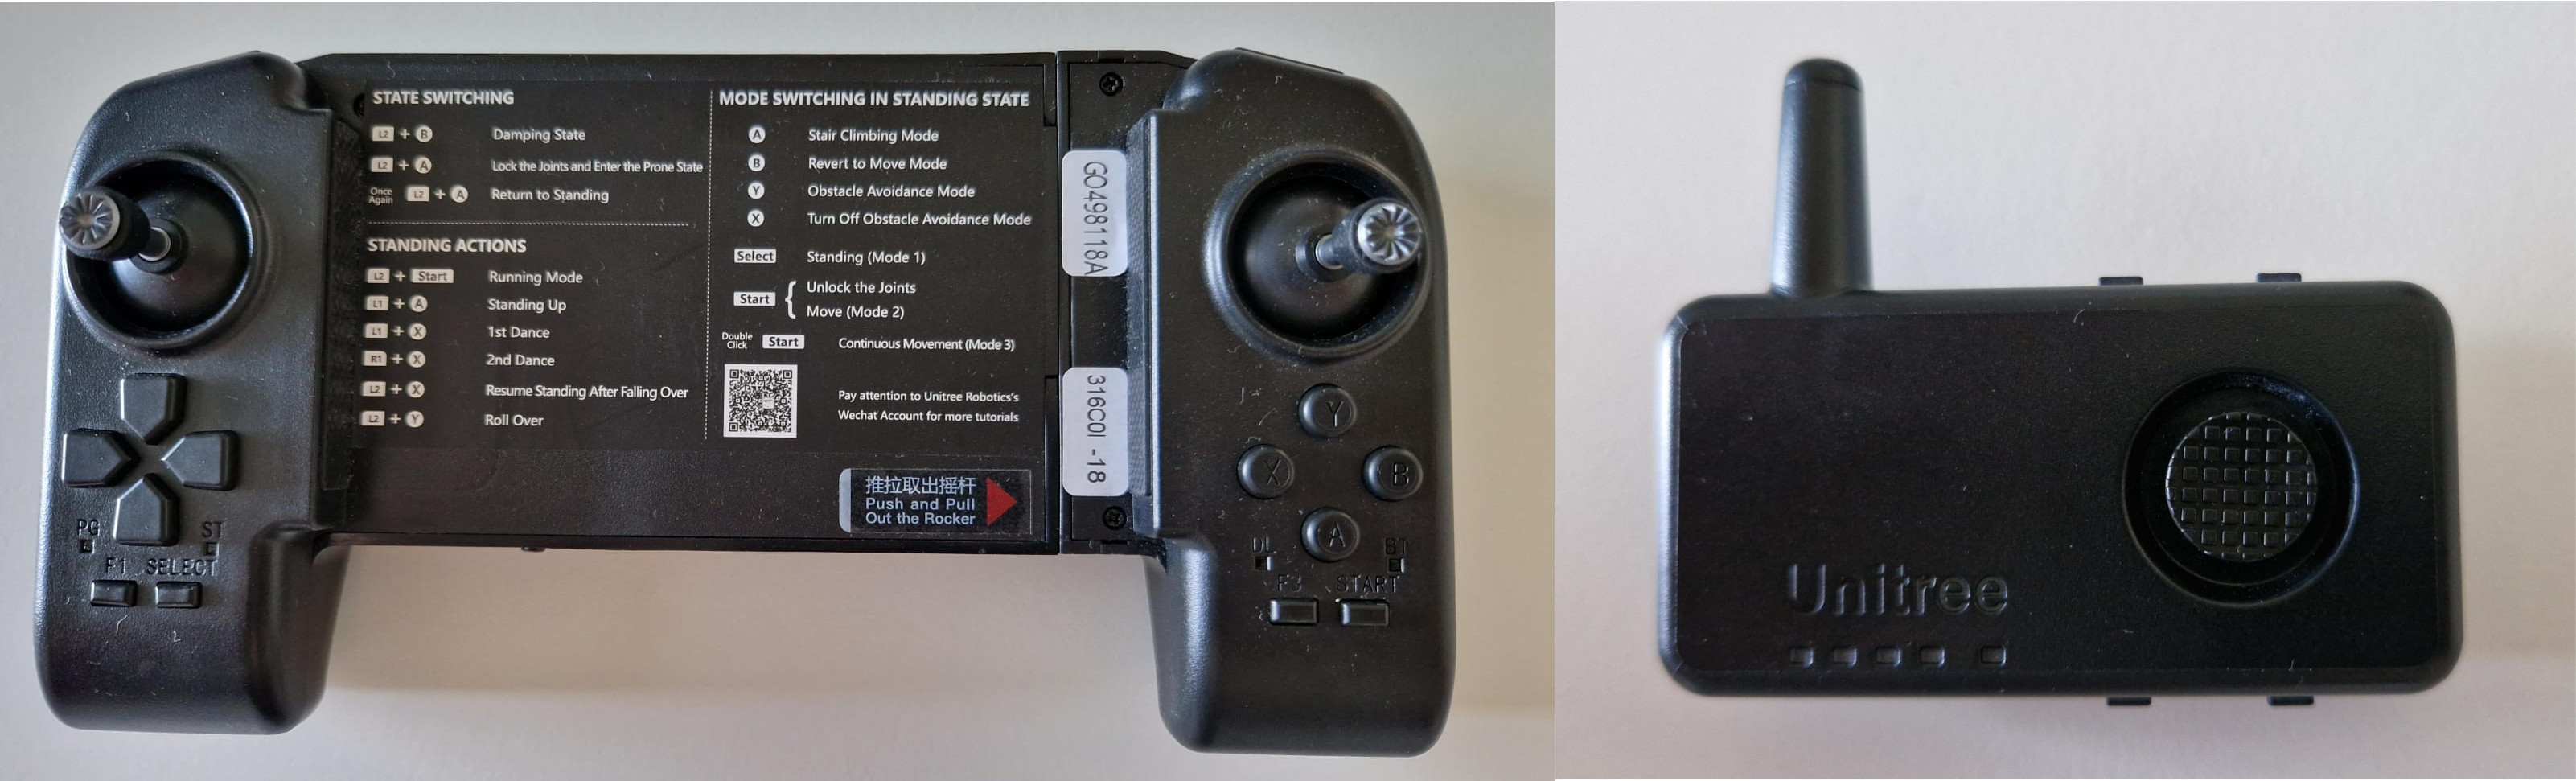
\includegraphics[width=\linewidth]{img/analyse/controller}}
    \caption{Hauptfernbedienung (links) und Label-Controller (rechts)}\label{fig:controller}
\end{figure}

Die einfache Bedienung der Hauptfernbedienung ist bereits nach dem Anschalten des Roboters nach Kapitel \ref{subsubsec:inbetriebnahme_akku} möglich.
Hierbei koppelt sich die Fernbedienung automatisch mit dem Roboter.
Dokumentation über die Art der Verbindung ist nicht auffindbar, es wird jedoch vermutet, dass dies nicht über Bluetooth,
sondern über ein anderes Protokoll geschieht und sich die Fernbedienung mit der \gls{mcu} statt mit dem Raspberry
Pi verbindet, welcher auch über Bluetooth verfügen würde.
Es beseht jedoch die Möglichkeit, die Fernbedienung via Bluetooth mit einem Smartphone zu koppeln.
Hierfür muss zur Verifikation der Kopplung der Pin \num{1234} verwendet werden.
Der Kopplungsprozess ist unter den verschiedenen Herstellern unterschiedlich und wird deshalb hier nicht weiter dokumentiert.
Nach erfolgreicher Kopplung kann über die mobile App\footnote{Siehe Kapitel \ref{subsubsec:anwendungen}} die Fernbedienung verbunden werden.
Über die Einstellungen und den Menüpunkt \texttt{Peripherals > Bluetooth Gamepad} kann in der Liste \texttt{Gamepad List}
die Fernbedienung mit der übereinstimmenden Seriennummer ausgewählt werden.
Diese ist ab Werk auf den Fernbedienungen gelabelt.
Abbildung \ref{fig:controller-app} zeigt die Bildschirmaufnahmen der relevanten Menüpunkte der App.

\begin{figure}[h]
    \frame{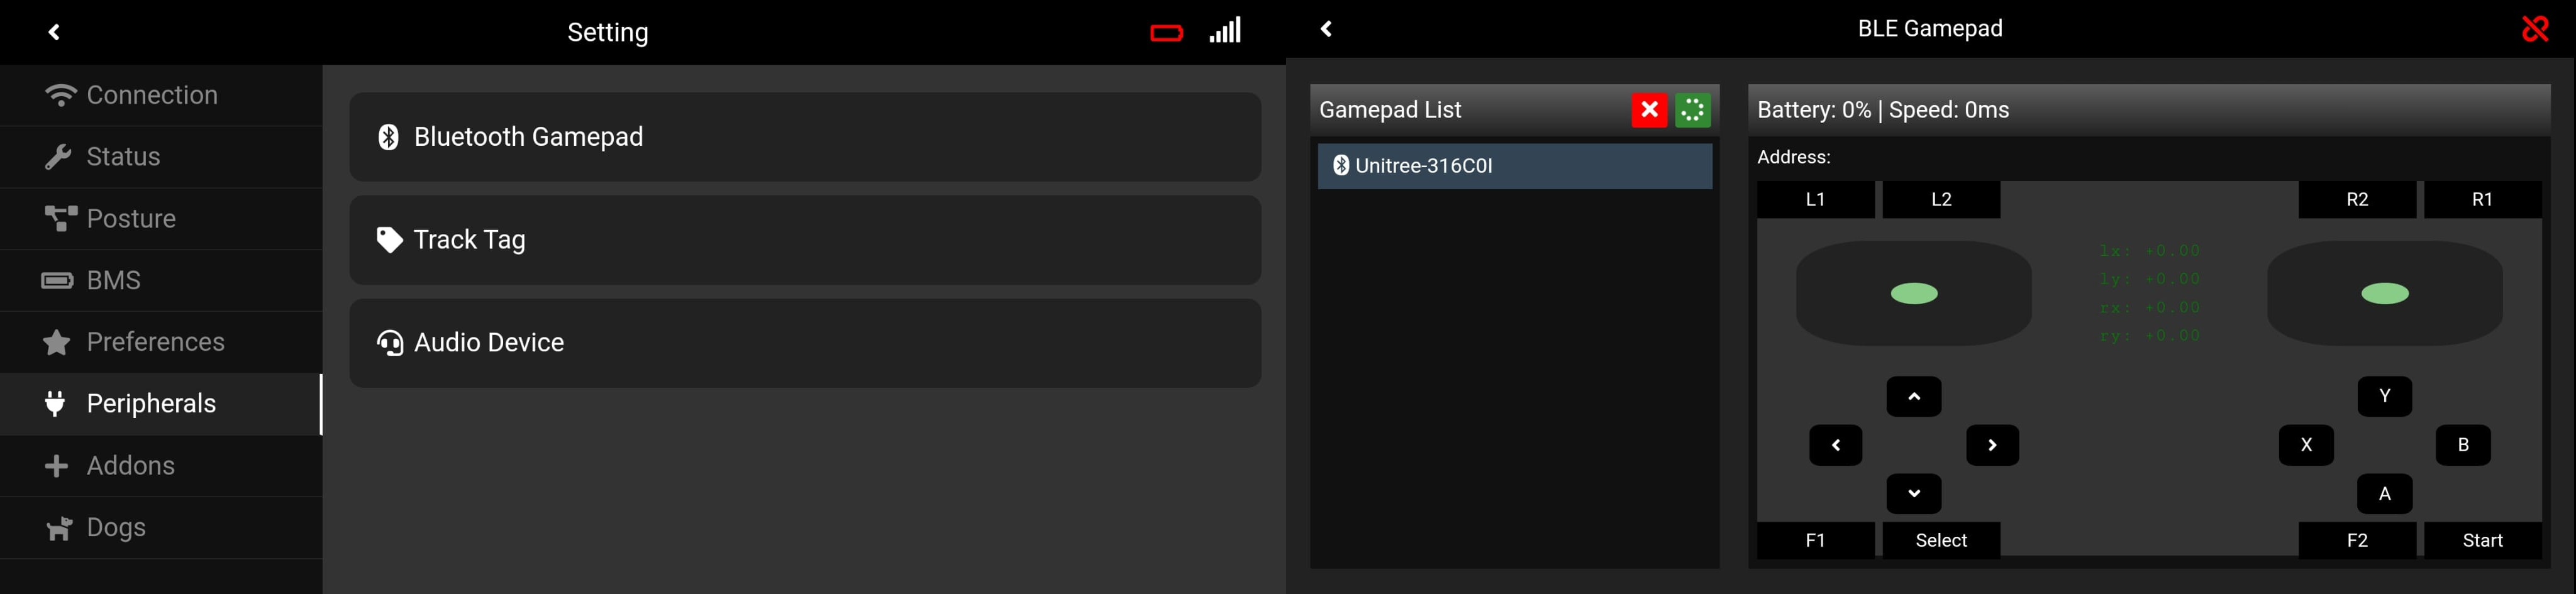
\includegraphics[width=\linewidth]{img/analyse/controller-app}}
    \caption{App-Menüpunkte \texttt{Peripherals > Bluetooth Gamepad} und \texttt{Gamepad List}}\label{fig:controller-app}
\end{figure}

\noindent Nun besteht die Möglichkeit, den \gls{go1} über die Fernbedienung fernzusteuern, egal in welchem Netzwerk er sich befindet.
Es ist lediglich notwendig, dass sich der Roboter und das Handy im selben Netzwerk befinden.
Weitere Informationen zur Netzwerkerweiterung sind in Kapitel \ref{sec:funktionserweiterungen-und-integration} dokumentiert.

\myparagraph{App}

Der \gls{go1} lässt sich ebenfalls durch die mobile Anwendung steuern, ohne sie vorher mit der Hauptfernbedienung verbunden zu haben.
Hierfür muss der Hauptmenüpunkt \texttt{Vision} ausgewählt werden.
Danach muss im rechten oberen Eck die Steuerung in der Ansicht der Kameras aktiviert werden.
Wie auf Abbildung \ref{fig:app-controller} gezeigt kann dann der Modus im rechten unteren Eck des Bildschirmes gewählt werden.
Wählt man hier einen der Laufmodi aus, so lässt sich der \gls{go1} mit den beiden dargestellten Steuereinheiten bewegen.
Links stellt die linke Steuereinheit der Hauptfernbedienung dar, rechts die rechte Einheit.

\begin{figure}[h]
    \frame{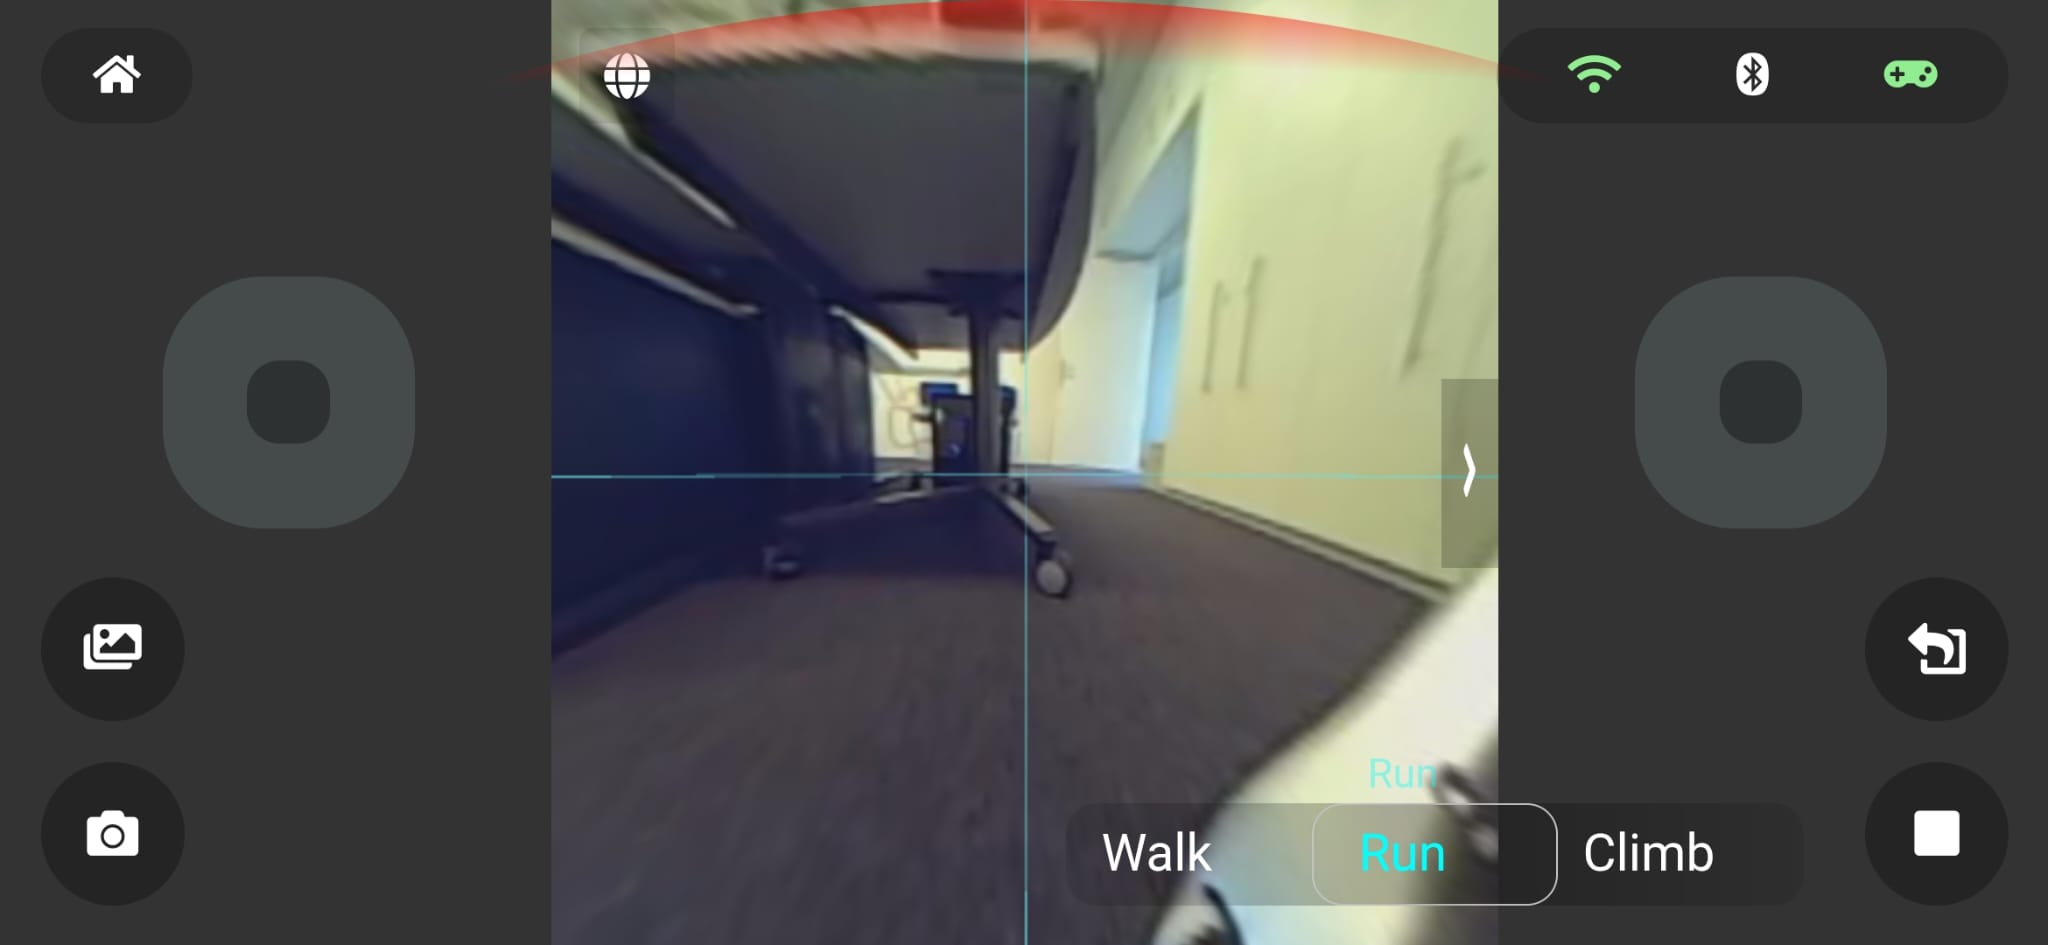
\includegraphics[width=\linewidth]{img/analyse/app-controller}}
    \caption{Bildschirmaufnahme des App-Controllers}\label{fig:app-controller}
\end{figure}

\myparagraph{Webinterface}

Die Webseite, die auf dem Raspberry Pi gehostet wird, bieter im Menü \texttt{Vision} die Möglichkeit, im rechten
oberen Eck des Bildschirmes die Steuerung des Roboters zu aktivieren.
Nach Aktivierung werden dem Nutzer, wie auf Abbildung \ref{fig:web-controller} dargestellt, zwei Steuerelemente dargestellt.
Diese können links mit den Tasten \texttt{W-A-S-D} und rechts mit den Tasten \texttt{\textuparrow -\textleftarrow -\textdownarrow -\textrightarrow}
gesteuert.
Die linke Steuereinheit entspricht der linken Seite der Hauptfernbedienung, die rechte dementsprechend der rechten Seite.

\begin{figure}[h]
    \frame{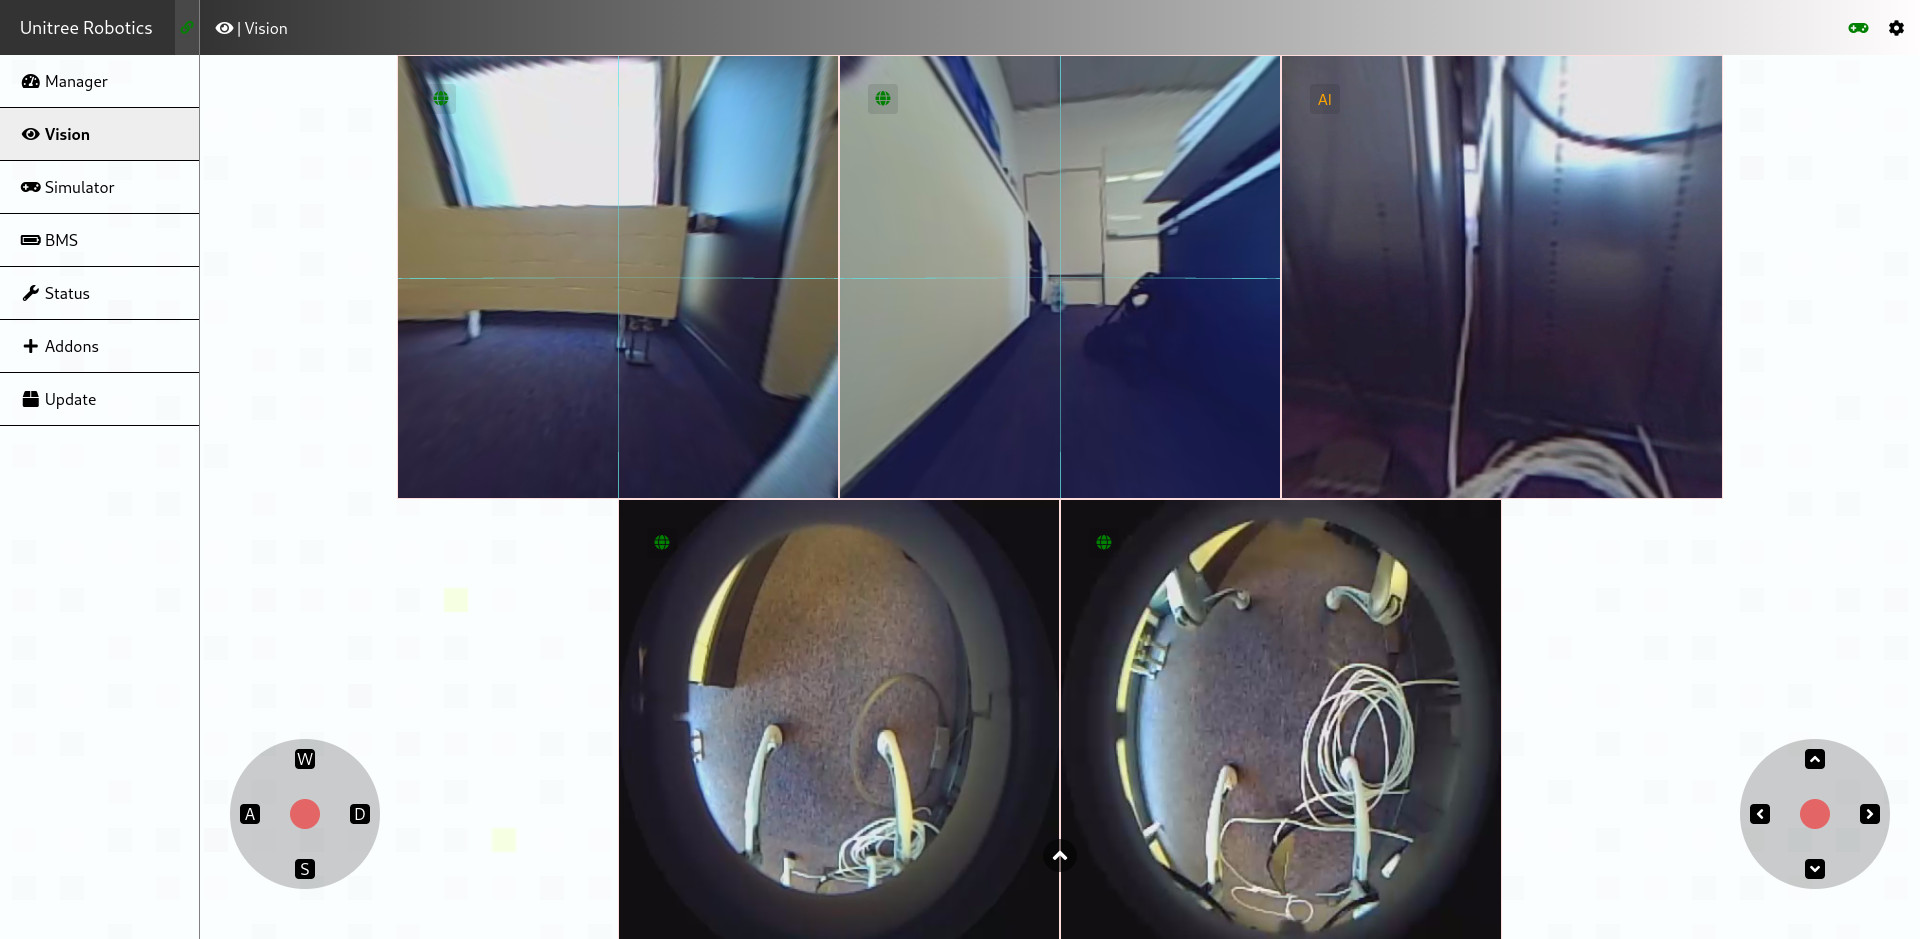
\includegraphics[width=\linewidth]{img/analyse/web-controller}}
    \caption{Bildschirmaufnahme des Web-Controllers}\label{fig:web-controller}
\end{figure}

\myparagraph{Folgefunktion}

Der sogenannte Label-Controller lässt sich genauso wie die Hauptfernbedienung über die Tastenkombination Drücken und
erneutes Drücken und Halten des \texttt{POW}-Knopfes anschalten.
Mit dem Joystick lässt sich der Roboter vereinfacht Steuern.
Die eigentliche Funktion des Label-Controllers ist jedoch die von Unitree Robotics \emph{Follow Me} Funktion.
Der Controller kommuniziert ständig mit dem Roboter und tauscht Informationen zur angenäherten Position des \gls{go1} relativ
zum Label-Controller aus.
Dies lässt sich in der mobilen App beobachten.
Hierfür muss über die Einstellungen auf den Pfad \texttt{Peripherals > Track Tag} navigiert werden.
Abbildung \ref{fig:follow-me} zeigt die beiden Bildschirmaufnahmen.

\begin{figure}[h]
    \frame{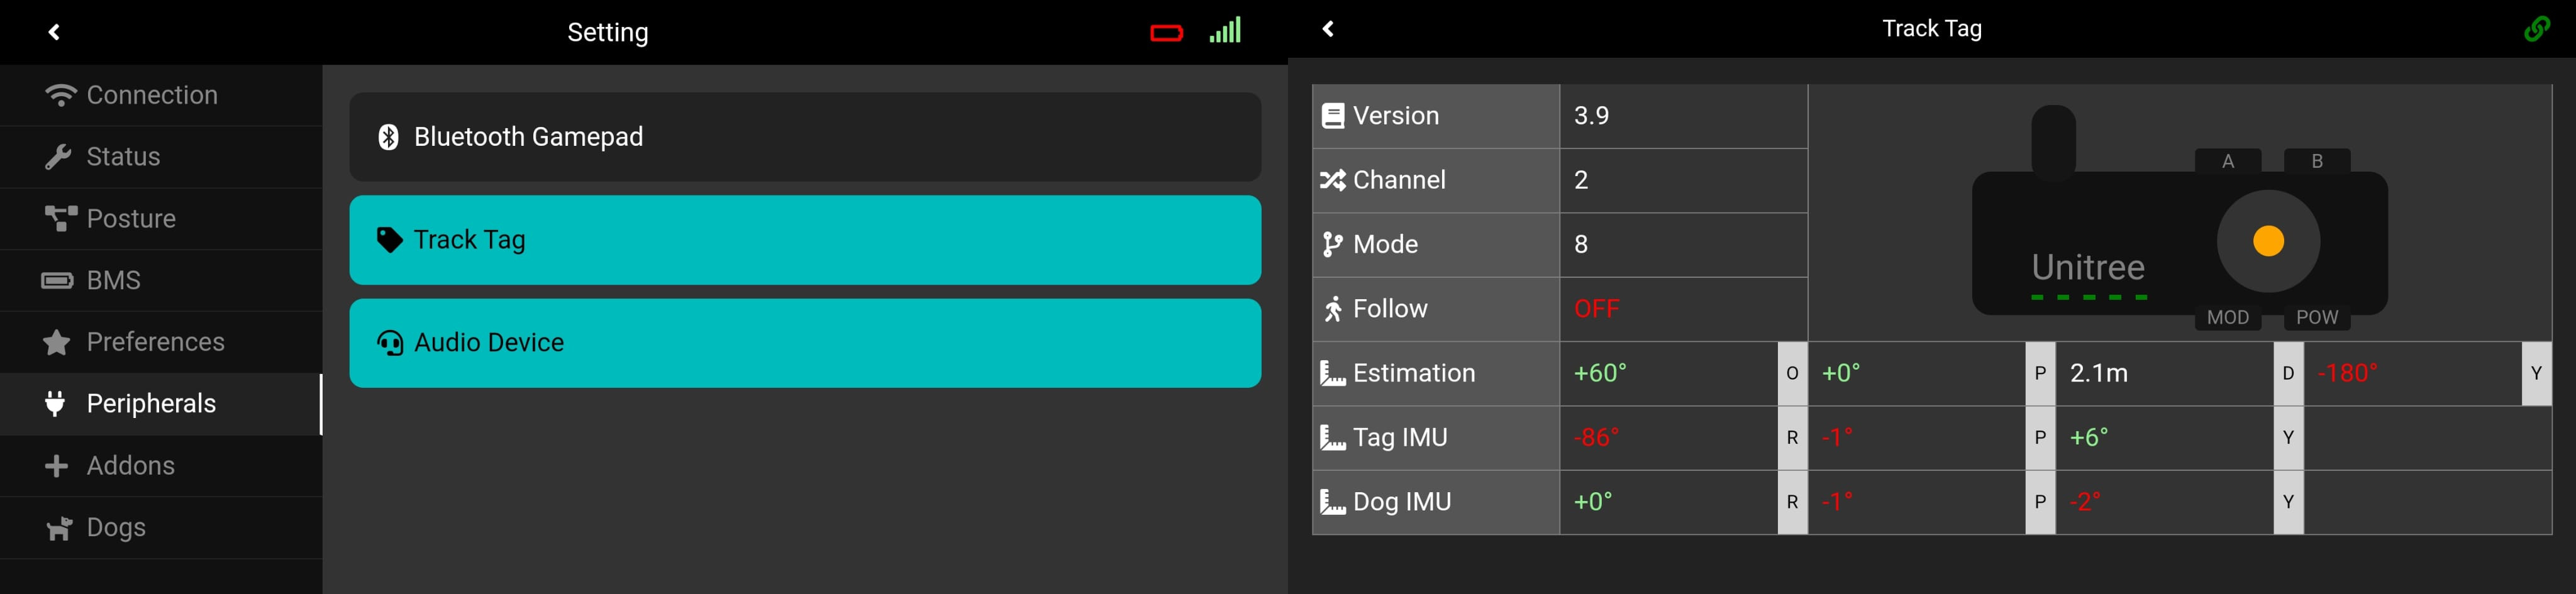
\includegraphics[width=\linewidth]{img/analyse/follow-me}}
    \caption{App-Menüpunkte \texttt{Peripherals > Track Tag} und die Tracking-Übersicht}\label{fig:follow-me}
\end{figure}

Um den Roboter zum Folgen zu bringen, muss der Wert der Option \texttt{Follow} angetippt werden.
Dieser sollte nun von \texttt{OFF} auf \texttt{ON} wechseln.
Danach bewegt sich der Hund immer relativ zum Label-Controller.
Durch die Tasten des Label-Controllers lässt sich das verhalten minimal anpassen.

\begin{table}[h]
    \centering
    \begin{tabular}{|c|l|}
        \hline
        \textbf{Taste} & \multicolumn{1}{c|}{\textbf{Funktion}} \\ \hline
        POW & \begin{tabular}[c]{@{}l@{}}\num{1} Sekunde Drücken \textrightarrow Aufrichten nach Sturz\\ \num{2} mal kurz Drücken \textrightarrow Wechsel der Standmodi\\ Stehen \textrightarrow Legen \textrightarrow Motoren deaktivieren \textrightarrow Stehen\end{tabular} \\ \hline
        MOD & \begin{tabular}[c]{@{}l@{}}Kurzes Drücken \textrightarrow Folgen deaktivieren\\ \num{2} mal kurz Drücken \textrightarrow Wechsel der Modi\\ Langsames Folgen (\num{1,5} m/s) \textrightarrow Schnelles Folgen (\num{3} m/s)\end{tabular} \\ \hline
        A & Wechsel Ausweichmodus (nach Test nicht Funktionsfähig) \\ \hline
        B & \begin{tabular}[c]{@{}l@{}}Kurzes Drücken \textrightarrow Rotation gegen Uhrzeigersinn um etwa 6\textdegree \\ \num{2} mal kurz Drücken \textrightarrow Reset der Rotation auf Standardwert\end{tabular} \\ \hline
    \end{tabular}\label{tab:label-controller-tasten}
\end{table}

\noindent Anzumerken ist, dass der Label-Controller nicht per Bluetooth mit dem Handy verbunden werden kann.
